\chapter{Konvoluční neuronové sítě}
\label{sec:CNN}

I když byly jedny z prvních NN použity ke zpracování obrazu, brzy se ukázalo,
že pro zpracování obrazu s větším rozlišením a větším množstvím kanálů je
klasická architektura NN velmi neefektivní. Bylo tedy třeba vytvořit jinou
architekturu, která by efektivně zpracovávala obrazová data. Nejznámější
takovou architekturou je konvoluční neuronová síť (ang. convolutional neural
network - CNN), která bude popsána v této kapitole.

\section{Problémy zpracování obrazu pomocí klasických neuronových sítí}

Klasickým přístupem pro zpracování obrazů pomocí neuronové sítě je vytvoření
sítě se stejným počtem prvků vstupní vrstvy, jako je počet pixelů vstupního
obrazu (za předpokladu jednoho kanálu). Tato vrstva je pak plně propojena s
několika skrytými vrstvami, výstupní vrstva pak buď vrací kategorie, v případě
klasifikace, nebo hodnoty hledaných atributů, jako je lokalizace objektů či
souřadnice klíčových bodů, v případě regrese.

Problémem tohoto přístupu je rozměr vstupních dat takové sítě. Běžná velikost
obrazu v dnešní době dosahuje několika miliónů pixelů, tento počet je ale ještě
vynásoben počtem kanálů, většinou třemi (RGB). To znamená, že velikost vstupní
vrstvy sítě je velmi vysoká, a aby byla taková síť efektivní, musí mít větší
počet skrytých vrstev a neuronů v těchto vrstvách. Ve výsledku má taková síť
velký počet parametrů, které je třeba natrénovat. Trénování takové sítě je
možné, je ale velmi nepraktické. Bylo by potřeba velké množství trénovacích
dat, jinak by s velkou pravděpodobností došlo k přetrénování sítě. I kdyby ale
bylo k dispozici dostatečné množství trénovacích dat, bylo by jak trénování,
tak i používání sítě velmi výpočetně i paměťově náročné.

CNN se proto tento problém řeší tak, že se snaží zredukovat rozměr vstupních
dat pomocí konvolučních vrstev, které jsou schopny efektivně zpracovávat
obrazová data.

\section{Konvoluce}

V kontextu počítačové grafiky je konvoluce binární operace, kdy pro daný pixel
sečteme hodnoty pixelů v jeho okolí vynásobené váhami vyjádřenými maskou, která
se nazývá jádro konvoluce (ang. kernel). Výsledný obraz je taky nazýván
konvoluce. Z matematického pohledu se jedná o diskrétní dvourozměrnou konvoluci
- binární operaci diskrétních funkcí, která je definována následovně:

\begin{equation*}
    (h*f)(x,y)=\sum _{i=-k}^{k}\sum _{j=-k}^{k}h(x-i,y-j)\cdot f(i,j)
\end{equation*}

kde $h$ je vstupní obraz, $f$ je jádro konvoluce, velikost jádra je $2k+1
    \times 2k+1$, a $x$ a $y$ jsou souřadnice pixelu, ke kterému se jádro aplikuje.

Hodnota konvoluce na dané pozici je tedy suma součinů hodnot pixelů vstupního
obrazu a hodnot váh vyjádřených jádrem konvoluce položeným středem na danou
pozici, viz obrázek \ref{fig:convolution}. Nejčastěji je velikost jádra lichá,
jelikož je pak jednodušší určení středu jádra.

\begin{figure}[]
    \centering
    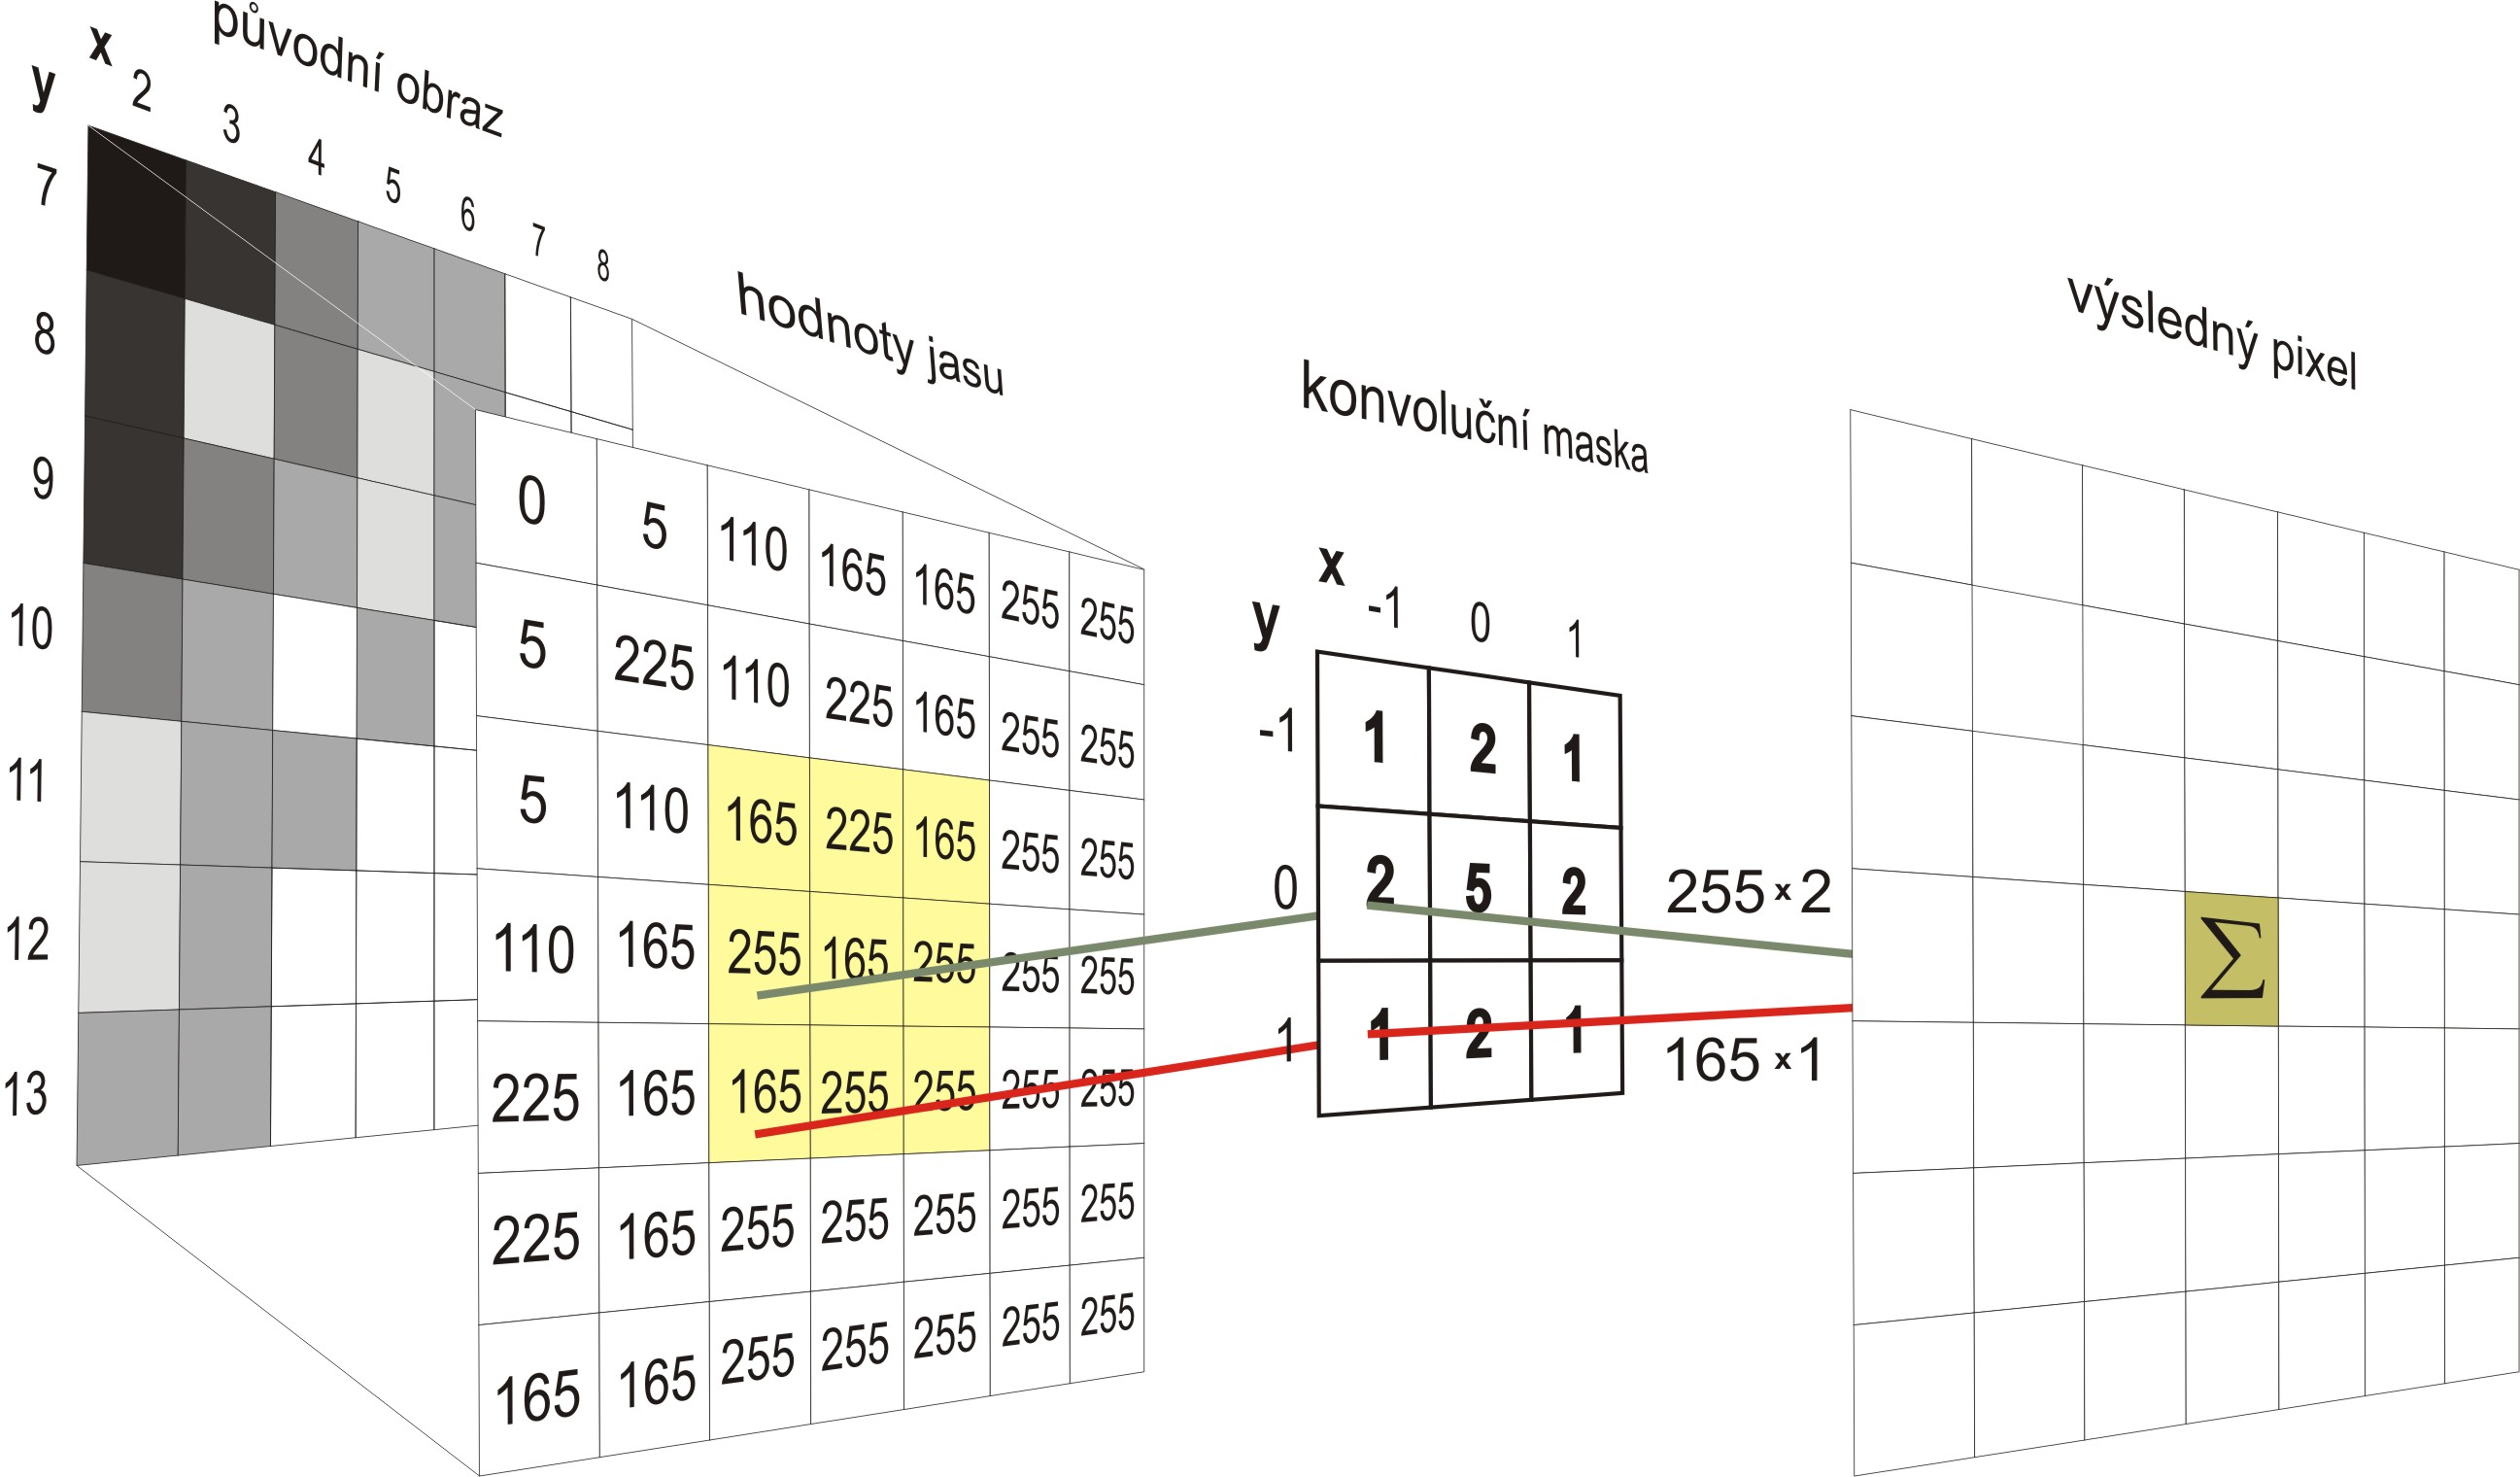
\includegraphics[width=0.8\textwidth]{Figures/convolution.jpg}
    \caption{Princip diskrétní dvourozměrné konvoluce \cite{}}
    \label{fig:convolution}
\end{figure}

Konvoluce je velmi rozšířená operace v počítačové grafice a zpracování obrazu,
k nejpoužívanějším aplikacím patří například rozmazání nebo detekce hran.

Pro rozmazání se používá například průměrovací filtr (ang. box blur)
využívající jádro, které má na všech pozicích hodnotu $1/n$, kde $n$ je počet
prvků jádra, viz obrázek \ref{fig:blur}. Výsledná hodnota konvoluce daného
pixelu je tedy rovná průměru hodnot tohoto pixelu a jeho sousedů. Dalším často
využívaným filtrem je Gaussovo rozostření, viz obrázek \ref{fig:blur}.
Rozmazání je někdy využíváno v počítačovém vidění jako první krok, za účelem
odstranění šumu z obrazu.

Pro detekci hran se často používá Sobelův operátor, který využívá dvě jádra -
pro vertikální a horizontální hrany. Jádra pro detekci hran jsou zobrazena na
obrázku \ref{fig:sobel}.

\begin{figure}[]
    \centering
    \begin{equation*}
        {\displaystyle {\frac {1}{9}}{
                \begin{bmatrix}
                    1 & 1 & 1 \\
                    1 & 1 & 1 \\
                    1 & 1 & 1 \\
                \end{bmatrix}},\ \ \ \ }
        {\displaystyle {\frac {1}{16}}{
                \begin{bmatrix}
                    1 & 2 & 1 \\
                    2 & 4 & 2 \\
                    1 & 2 & 1 \\
                \end{bmatrix}}}
    \end{equation*}

    \caption{Jádro konvoluce pro průměrovací a Gaussovo rozostření}
    \label{fig:blur}
\end{figure}
\begin{figure}[]
    \centering
    \begin{equation*}
        {\displaystyle {
                \begin{bmatrix}
                    -1 & 0 & 1 \\
                    -2 & 0 & 2 \\
                    -1 & 0 & 1 \\
                \end{bmatrix}},\ \ \ \ }
        {\displaystyle {
                \begin{bmatrix}
                    -1 & -2 & -1 \\
                    0  & 0  & 0  \\
                    1  & 2  & 1  \\
                \end{bmatrix}},\ \ \ \ }
    \end{equation*}

    \caption{Jádro konvoluce pro detekci vertikálních a horizontálních hran využívané pro Sobelův operátor}
    \label{fig:sobel}
\end{figure}

V případě více kanálů vstupního obrazu musí být připraveno zvlášť jádro pro
každý kanál. Výsledné konvoluce se pak sečtou. Můžeme se na tuto situaci dívat
i jako na třírozměrné konvoluční jádro s rozměrem třetí dimenze rovným počtu
kanálů vstupního obrazu. Konvoluce je pak prováděná tak, že na každé pozici
vstupního obrazu provedeme součet vah jádra vynásobených hodnotami vstupního
obrazu na příslušných pozicích napříč všemi kanály. Výstup takové konvoluce má
pouze jeden kanál.

Myšlenkou konvolučních neuronových sítí je nahradit plně propojené vrstvy
konvolučními vrstvami. Ruční nastavení všech hodnot jader tak, aby konvoluční
vrstvy extrahovaly požadované vlastnosti z obrázku, je ale velmi obtížné, v
případě složitějších či obecnějších problémů téměř nemožné. V 1989 proto Yann
LeCun et al. navrhli metodu, jak se síť může hodnoty jader naučit sama, a tak
si efektivně vytvořit i složitější filtry, které by člověk těžko navrhl ručně.
Zjistili, že váhy konvolučních jader se mohou trénovat pomocí algoritmu
backpropagation stejně jako váhy neuronů v plně propojených vrstvách.

Takový přístup má mnoho výhod. Konvoluce se dá velmi dobře paralelizovat a
zajistit tak vysokou efektivitu výpočtů. Oproti plně propojeným vrstvám má vždy
konvoluce s jedním jádrem počet vah pouze rovný velikosti jádra. I v případě
provedení mnoha konvolucí je počet výrazně menší než v případě potřebného počtu
a velikosti plně propojených vrstev. Zároveň lze pomocí konvolucí efektivně
extrahovat různé vlastnosti ze vstupního obrazu, ty pak pomocí plně propojených
vrstev zpracovat a využít k řešení problému. Proto se taky výstupu konvoluce
často říká mapa příznaků (ang. feature map).

\section{Krok a padding}

Pro pochopení funkčnosti konvolučních neuronových sítí je ještě důležité
pochopit dva parametry, které ovlivňují výstup konvoluční vrstvy. Jedná se o
krok (ang. stride) a padding (česky vycpávka či doplnění).

Krok určuje, co kolik pixelů se aplikuje jádro konvoluce na vstupní obraz.
Pokud tedy bude krok $k = 1$, bude jádro aplikováno na každý pixel vstupního
obrazu. Pokud bude krok $k = 2$, bude jádro aplikováno na každý druhý pixel
vstupního obrazu. Pokud bude krok $k > 1$, bude výstup konvoluce násobně menší.

Jelikož na nejkrajnější pixely nemůžeme aplikovat jádro, protože by přesahovalo
hranice obrazu, bude se obraz z každou konvolucí nežádaně zmenšovat i při
jednotkovém kroku. Pokud použijeme například jádro o velikosti $3 \times 3$,
bude výsledná mapa o 2 řádky a 2 sloupce menší, než byl vstupní obraz. Dalším
problémem je, že ve výsledné konvoluci je marginalizován vliv krajních pixelů.
Obraz je tedy jistým způsobem oříznut. Tyto problémy se proto někdy řeší pomocí
tzv. paddingu. Je to technika, kdy se vstupní obraz rozšíří o takový počet
pixelů z každé strany, aby vzhledem k velikosti konvolučního jádra bylo možné
aplikovat jádro i na krajní pixely obrazu.

Velikost výstupní mapy konvoluce je tedy dána vztahem:

\begin{equation*}
    \left\lfloor \frac{n+2p-f}{s}+1 \right\rfloor \times \left\lfloor \frac{n+2p-f}{s}+1 \right\rfloor
\end{equation*}

kde $n$ je velikost vstupního obrazu, $p$ je velikost paddingu, $s$ je krok a
jádro je velikosti $f \times f$.

\section{Konvoluční vrstva}

Konvoluční vrstva je základním prvkem konvoluční neuronové sítě. V jistém slova
smyslu je podobná plně propojené vrstvě, jelikož obsahuje váhy, biasy a
aktivační funkce. Namísto plného propojení s neurony následující vrstvy je ale
aplikována konvoluce na vstupní data. K výstupní mapě je přičten bias a
následně může být aplikována aktivační funkce.

Jedná vrstva může mít několik konvolučních jader, každé s vlastními váhami a
biasem. Je třeba zároveň pamatovat, že každé jádro musí mít hloubku rovnou
počtu vstupních map, resp. počtu kanálu vstupního obrazu v případě vstupní
vrstvy. Konvoluci pak aplikujeme zvlášť pro každé jádro, počet výstupních map
příznaků tedy bude roven počtu jader v dané vrstvě. V praxi bude každé jádro
vyjadřovat jinou vlastnost, kterou se snažíme ze vstupního obrazu extrahovat.

Množinu parametrů dané konvoluční vrstvy tedy tvoří hodnoty jader a jejích
příslušné biasy. K hyperparametrům pak patří počet jader a jejich velikost,
aktivační funkce, krok a padding.

\section{Poolovací vrstva}
Jak již bylo zmíněno, v konvolučních vrstvách vzniká vícero map příznaků
vyjadřující různé vlastnosti. Tím se ale množství dat zvětšuje, což porušuje
samotnou myšlenku konvolučních sítí, která je založena na snaze zredukovat
rozměr dat. Proto se snažíme rozměr map příznaků zmenšovat. Jak již bylo
zmíněno, dojde k redukci rozměrů v konvoluční vrstvě, pokud použijeme krok $k >
    1$. Častěji ale je k tomuto účelu prováděno podvzorkování dat v tzv.
poolovacích vrstvách (z ang. pooling layer).

V poolovací vrstvě je vstupní mapa rozdělená do stejně velkých čtvercových
oblastí velikosti $t \times t$, na základě hodnot v daném čtverci je pak
vytvořen jeden pixel výstupní mapy. K nejčastěji používaným metodám patří
max-pooling a average-pooling. Max-pooling vybere z dané oblasti největší
hodnotu, zatímco average-pooling vyhodnotí z každé oblasti průměr hodnot.
Velikost výstupní mapy pro vstup velikosti $n \times n$ a poolovací oblasti
velikosti $t \times t$ je tedy $\left\lfloor \frac{n}{t} \right\rfloor \times
    \left\lfloor \frac{n}{t} \right\rfloor$.

\section{Architektura CNN}

Konvoluční neuronové sítě se skládají ze dvou částí - konvoluční části a plně
propojené části.

Konvoluční část se skládá z několika konvolučních vrstev proplétaných s
poolovacími vrstvami. V této části se pracuje s mapami příznaků. Její výstupem
je soubor map příznaků, resp. mapa příznaků s větší hloubkou, která vyjadřuje
různé vlastnosti vstupního obrazu.

Plně propojená část je pak klasická dopředná neuronová síť, která na základě
extrahovaných vlastností provádí klasifikační či regresní úlohu. Před vstupem
do plně propojené části jsou mapy příznaků převedené do jednoho vektoru o
velikosti rovné součtu velikostí všech map příznaků.

\endinput
